\chapter{Simulation}
In this project it was simulated a Pressurized Water Reactor (PWR) with different Thorium fuel cycles. The simulation aims to understand the behavior of thorium based nuclear fuels in a PWR. 

\section{Methodology}
The simulation was done using openMC, which is a library for Monte Carlo simulations of neutron transport. The code was developed by the Computational Reactor Physics Group (CRPG) at the Massachusetts Institute of Technology (MIT). 

\subsection{Monte Carlo Method}
The Monte Carlo method is a statistical technique used to solve mathematical problems by generating random samples to obtain numerical results. This method simulates a large number of individual particles and their interactions with materials, then estimates the desired quantities by averaging the results of all particles \cite{TMSR_book}.

The simulation code is written in Fortran 2008 and uses the FoX XML library to process input files in XML format \cite{OpenMC}. XML is used for all inputs because it allows developers to easily modify options, and the FoX library efficiently handles these changes as long as the file structure is well-defined and consistent with the specification files \cite{OpenMC}.

\subsection{OpenMC}
The input files are divided into three mandatory categories for every simulation: settings, materials, and geometry. The settings file contains all simulation parameters, including the number of particles to run. The materials file describes the composition of the materials by densities and elements or nuclei. The geometry file defines the model's geometry \cite{OpenMC}.

However, it is needed to set an additional environment variable to run the code. The environment variable is called ``\texttt{OPENMC\_CROSS\_SECTIONS}'' and it is used to specify the path to the cross-section data. The cross-section data is a library that contains the cross-sections for all isotopes used in the simulation. The library is generated using the ``NJOY'' nuclear data processing code. However, it is also possible to use the cross-section data from the official data libraries like ENDF/B-VII.1 \cite{OpenMC}.

The implemented code uses depletion calculations to simulate the evolution of the fuel composition over time. The depletion calculations are done using the OpenMC depletion capability. The library uses numerical integration to solve the coupled concentration equation known as bateman equations \cite{OpenMC}. Bateman equations are a series of differential equations that describe the time evolution of the concentration of isotopes in a nuclear reactor. The equations are given by:

\begin{flalign}
    && \frac{dN_i(t)}{dt} = \sum_{j} \left[ \int_{0}^{\infty} \sigma_{j \to i}(E,t)\phi(E, t)dE + \lambda_{j \to i} \right] N_{j}(t) && \nonumber \\
    && - \sum_{j} \left[ \int_{0}^{\infty} \sigma_{i \to j}(E,t)\phi(E, t)dE + \lambda_{i \to j} \right] N_{i}(t) &&
\end{flalign}

\vspace{0.5cm}

Where \(N_{i}(t)\) is the number of nuclei of isotope \(i\) at time \(t\), \(\sigma_{j \to i}(E,t)\) is the microscopic cross-section for the reaction where a nucleus of the kind \(j\) generates an isotope of the kind \(i\) \cite{Bateman_equation}. For the depletion calculations, it is necessary to give an additional input file that contains the transmutation reactions and the decay constants for the isotopes. The depletion file is also in XML format \cite{OpenMCweb}.

The results from the depletion calculations are stored in an output file in HDF5 format. The HDF5 format allows parallel writing of the data, make it possible multi threading execution, and is a widely used format for storing large amounts of data. The output file contains the number of nuclei of each isotope at each time step, the k-effective, and the neutron flux \cite{OpenMCweb,HDFGroupDoc}. Additional, information about the output file can be found in the OpenMC documentation \textbf{Ref.}\cite{OpenMCweb}.

\section{Model}
The model used in the simulation is a PWR. It was use the model from the OpenMC example files. The model is a \(17\times17\) fuel assembly from the ``BEAVRS'' benchmark. The model is a 3D model with 3 regions: fuel, water, and cladding. The fuel is a \(UO_2\) fuel with \(3.1 \, \%\) enrichment. The cladding is made of Zircaloy-4 and the water is light water (\(H_2O\)). 

The code is made of two main parts. The first part implements the assembly and defines the nuclear model. In this script settings like the number of particles, the number of batches, and the number of generations are defined. The second part is the depletion script. This script defines the depletion calculations and the output file.

Multiple file for plotting the results are also implemented. The files are written in Python and use the libraries ``numpy'', ``matplotlib'', and ``h5py''. The files read the output file from the depletion calculations and plot the results. The plots show the percentage change in each step of simulation of each isotope. Finally, the plots are saved in a directory called ``plots''. 

\subsection{Project Structure}

The project is organized into several directories and files, each serving a specific purpose:

\begin{tcolorbox}
    Root/: Project root directory.
    \begin{itemize}[itemsep=0pt, parsep=0pt]
        \item Data/: Data files for the simulation.
        \begin{itemize}[itemsep=0pt, parsep=0pt]
            \item \texttt{chain\_endfb80\_pwr.xml}
            \item ...
        \end{itemize}
        \item Plots/: Plot images from simulation results.
        \begin{itemize}[itemsep=0pt, parsep=0pt]
            \item \texttt{percentual\_change\_th232\_con\_10.pdf}
            \item ...
        \end{itemize}
        \item Results/: Simulation results.
        \begin{itemize}[itemsep=0pt, parsep=0pt]
            \item \texttt{Th232/}
            \item ...
        \end{itemize}
        \item Simulation/: Simulation scripts and files.
        \begin{itemize}[itemsep=0pt, parsep=0pt]
            \item \texttt{plotter\_3.py}
            \item \texttt{pwr\_model\_source.py}
            \item \texttt{run\_reactor.py}
            \item ...
        \end{itemize}
        \item \texttt{README.md}: Project documentation.
        \item \texttt{dockerfile}: Docker configuration.
    \end{itemize}
\end{tcolorbox}

The simulation directory contains the core Python scripts essential for the simulation process. The ``\texttt{pwr\_model\_source.py}'' script implements the detailed fuel assembly. The ``\texttt{run\_reactor.py}'' script manages the simulation execution. The ``\texttt{plotter\_3.py}'' script processes the simulation data, generating visual representations of the results. The data directory includes critical files such as depletion chain file. The results directory stores the output files from the simulations, sorting the generated data. 

\section{Results}
Multiple simulations were conducted to evaluate the behavior of the fuel during the operation of the PWR over a period of 6 months. Simulations were performed with various thorium concentrations in uranium oxide fuel, specifically \(10 \, \%\) and \(50 \, \%\). Figures \textbf{Fig.}\ref{fig:th10} and \textbf{Fig.}\ref{fig:th50} illustrate the results of these simulations, showing the percentage change of isotopes in the fuel assembly over the simulation period. The plots indicate the achievement of breeding in the fuel assembly for \(\prescript{233}{}{U}\). However, it is noticeable that the stability of breeding is achieved much later compared to \(\prescript{239}{}{Pu}\). This is expected since the breeding of \(\prescript{233}{}{U}\) follows the chain reaction of \(\prescript{232}{}{Th} \xrightarrow{\substack{\text{neutron} \\ \text{absorption}}} \prescript{233}{}{Th} \xrightarrow{22 \, \text{minutes}} \prescript{233}{}{Pa} \xrightarrow{27 \, \text{days}} \prescript{233}{}{U}\), which is a much slower breading process than the chain reaction of \(\prescript{238}{}{U} \xrightarrow{\substack{\text{neutron} \\ \text{absorption}}} \prescript{239}{}{U} \xrightarrow{23.5 \, \text{minutes}} \prescript{239}{}{Np} \xrightarrow{2.4 \, \text{days}} \prescript{239}{}{Pu}\) for plutonium breading.

\begin{figure}[h]
    \centering
    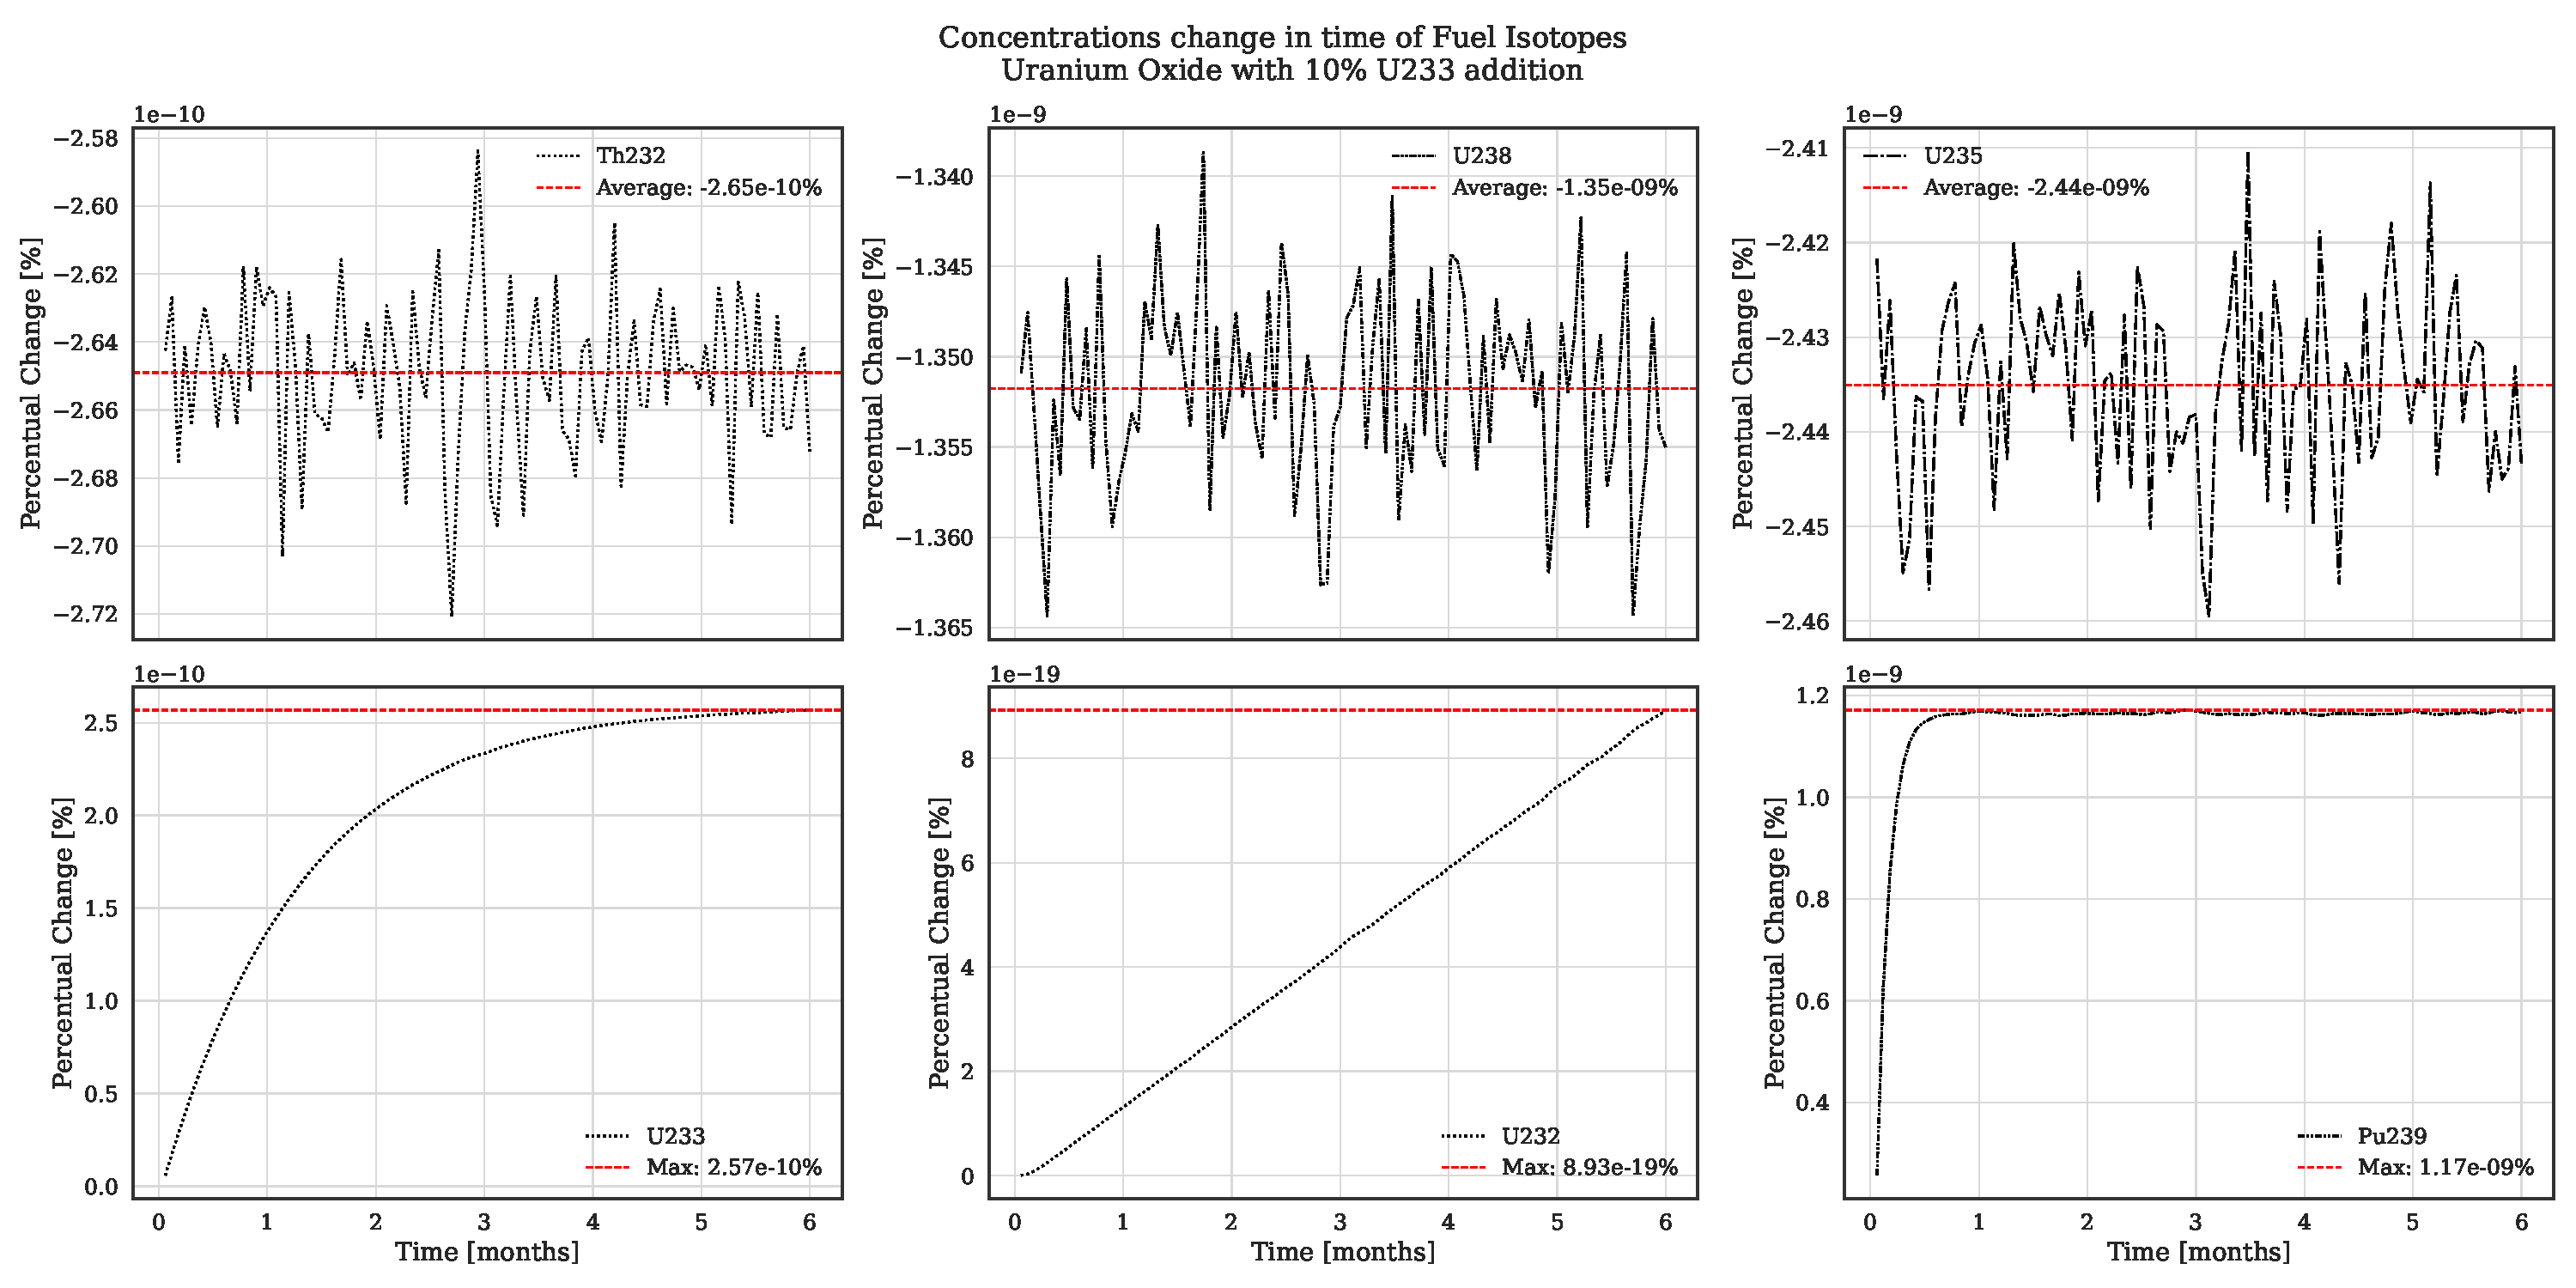
\includegraphics[width=1\textwidth]{Kap7/Figures_Kap7/percentual_change_th232_con_10.pdf}
    \caption{Percentage change of isotopes in the simulation of a PWR fuel assembly using UOX at \(10 \, \%\) thorium concentration.}
    \label{fig:th10}
\end{figure}

\begin{figure}[h]
    \centering
    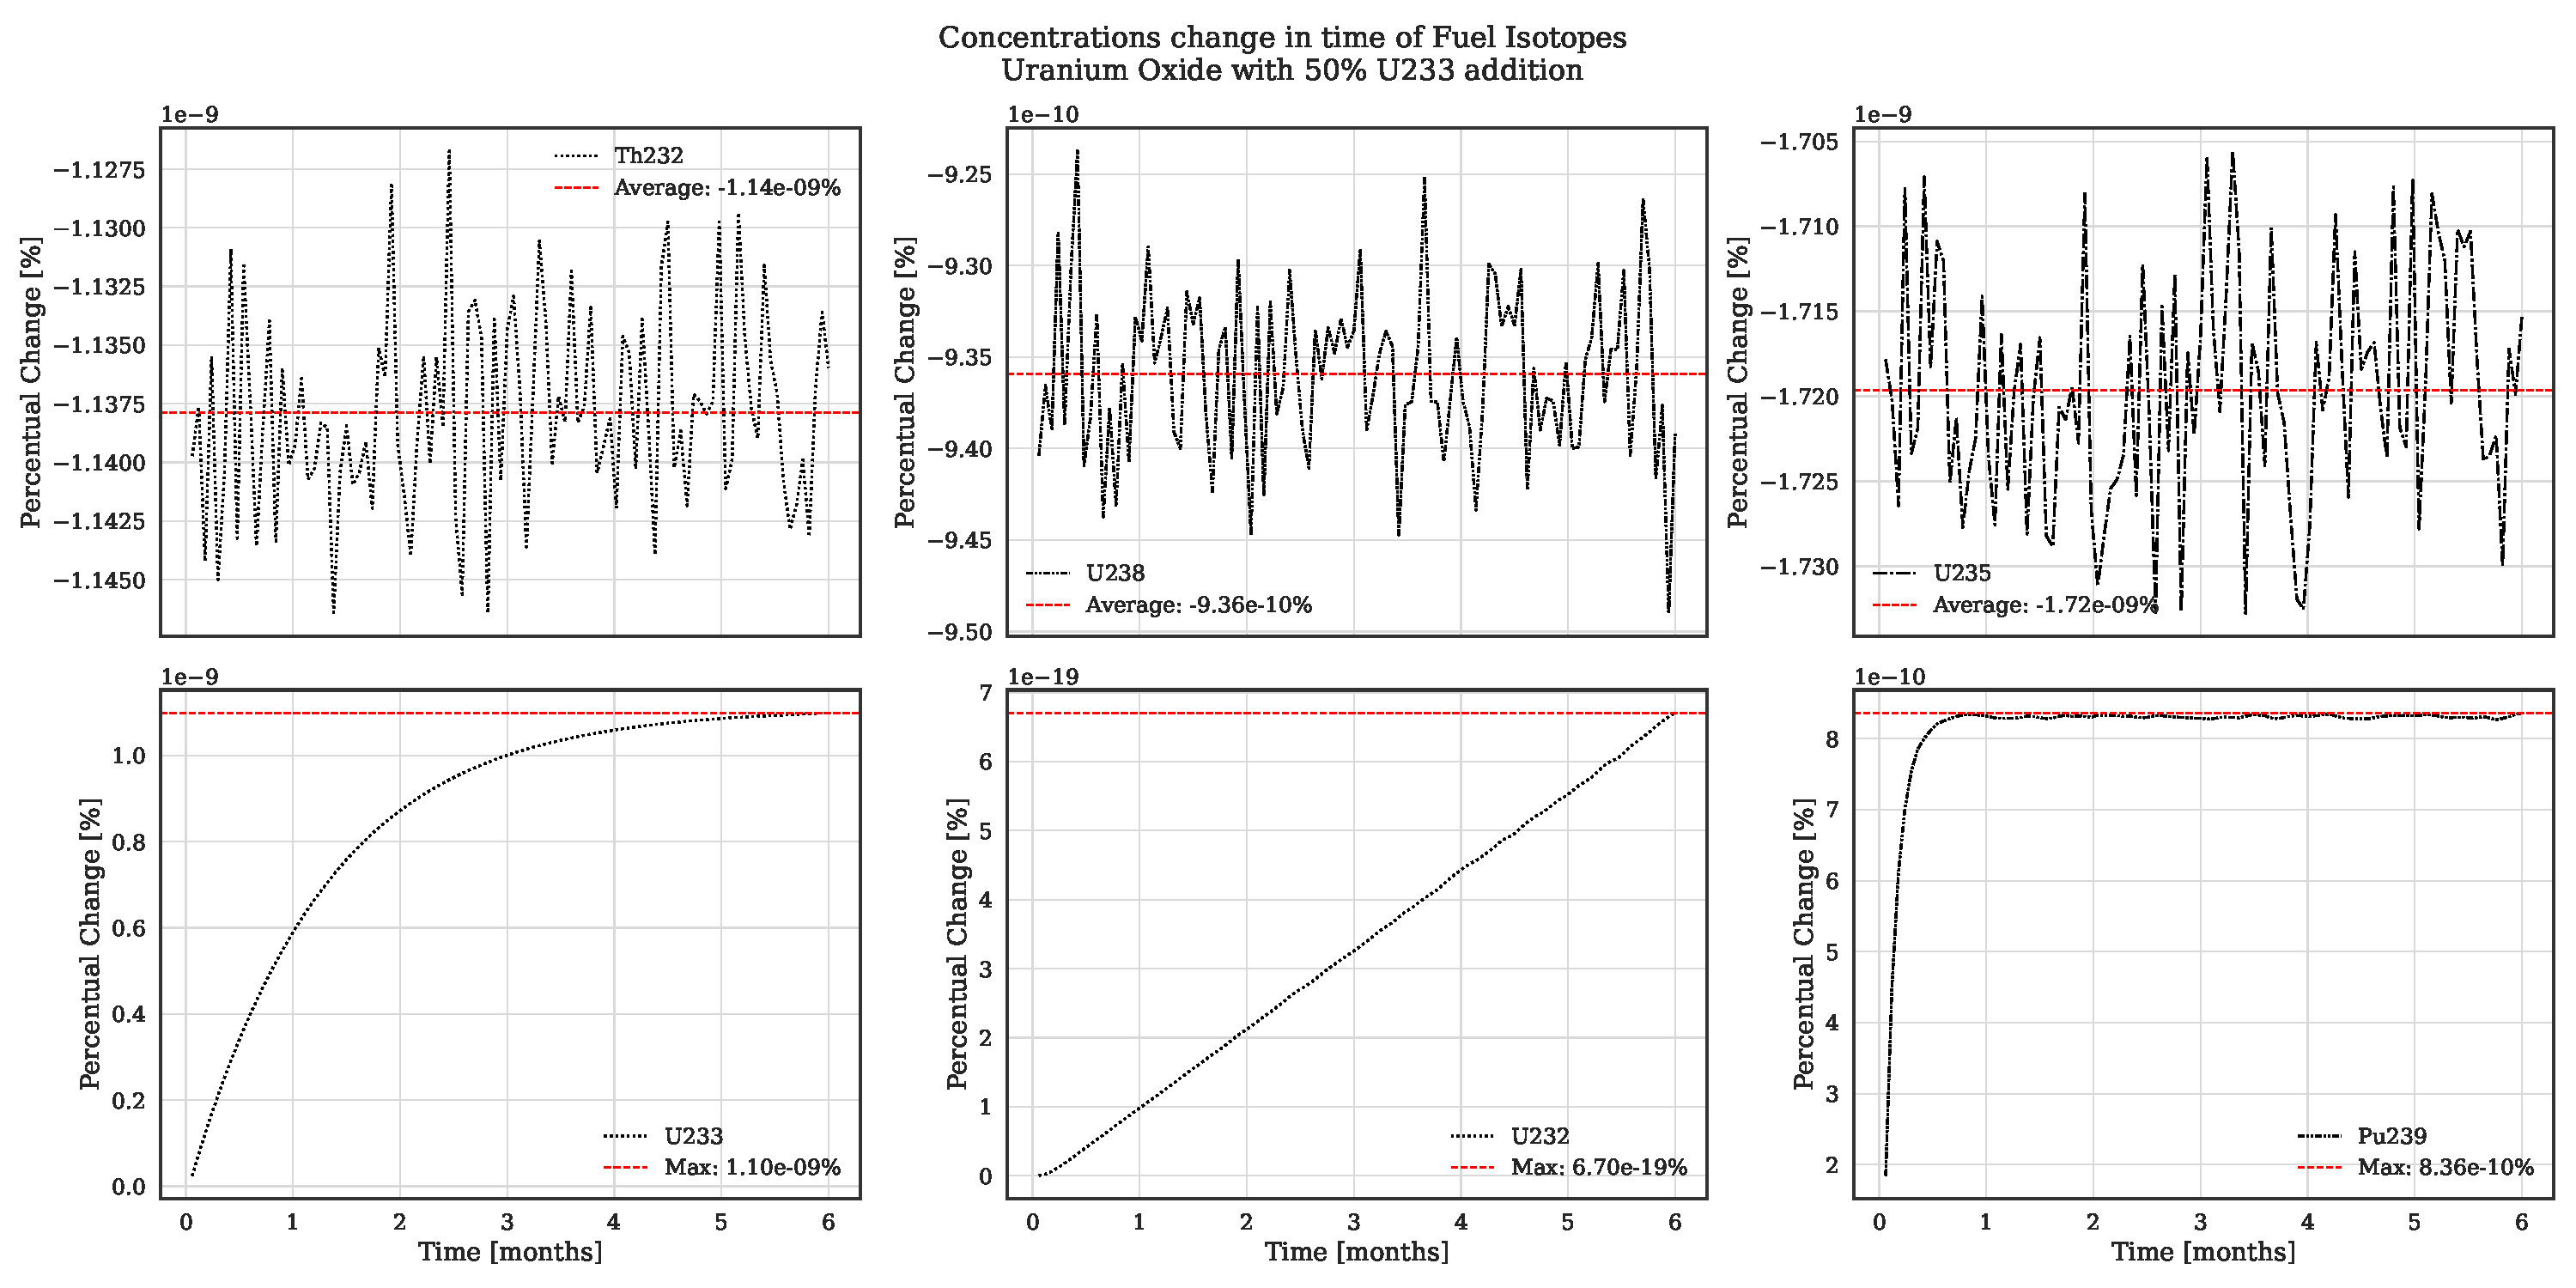
\includegraphics[width=1\textwidth]{Kap7/Figures_Kap7/percentual_change_th232_con_50.pdf}
    \caption{Percentage change of isotopes in the simulation of a PWR fuel assembly using UOX at \(50 \, \%\) thorium concentration.}
    \label{fig:th50}
\end{figure}

The simulations demonstrate that a \(10 \, \%\) thorium concentration in the fuel results in a good neutronic economy, aligning with previously reported results \cite{N_Improvement}. However, a \(50 \, \%\) thorium concentration leads to subcritical reactor behavior. This result are shown in figures \textbf{Fig.}\ref{fig:p_10} and \textbf{Fig.}\ref{fig:p_10}.

\begin{figure}[h]
    \centering
    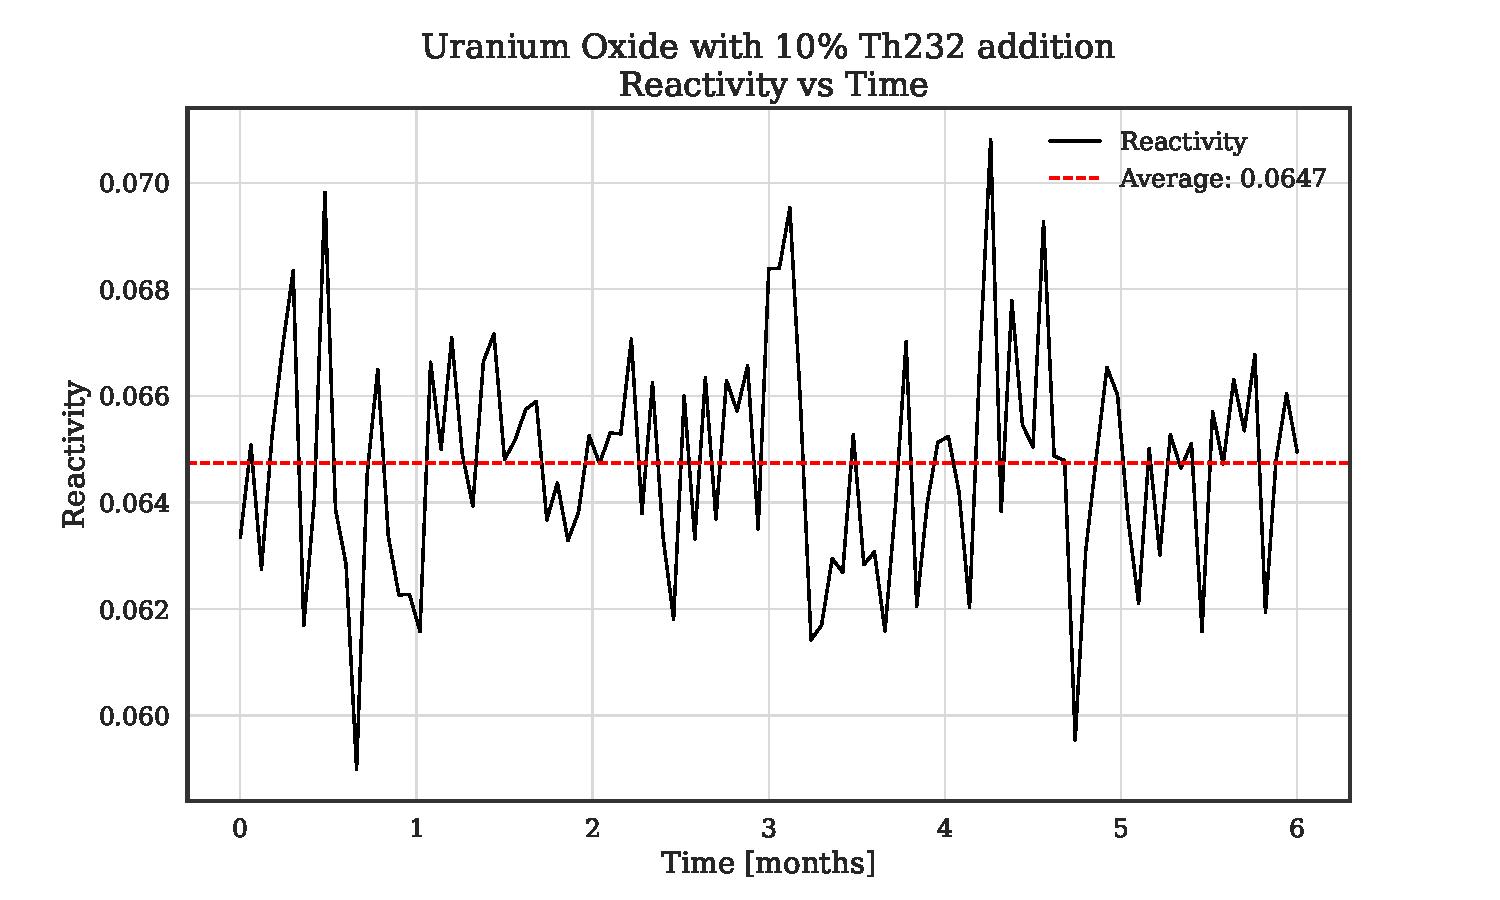
\includegraphics[width=0.75\textwidth, scale = 0.5]{Kap7/Figures_Kap7/Reactivity_vs_Time_UOX_10.pdf}
    \caption{Reactivity over time of the simulation of a PWR fuel assembly using UOX at \(10 \, \%\) thorium concentration.}
    \label{fig:p_10}
\end{figure}

\begin{figure}[h]
    \centering
    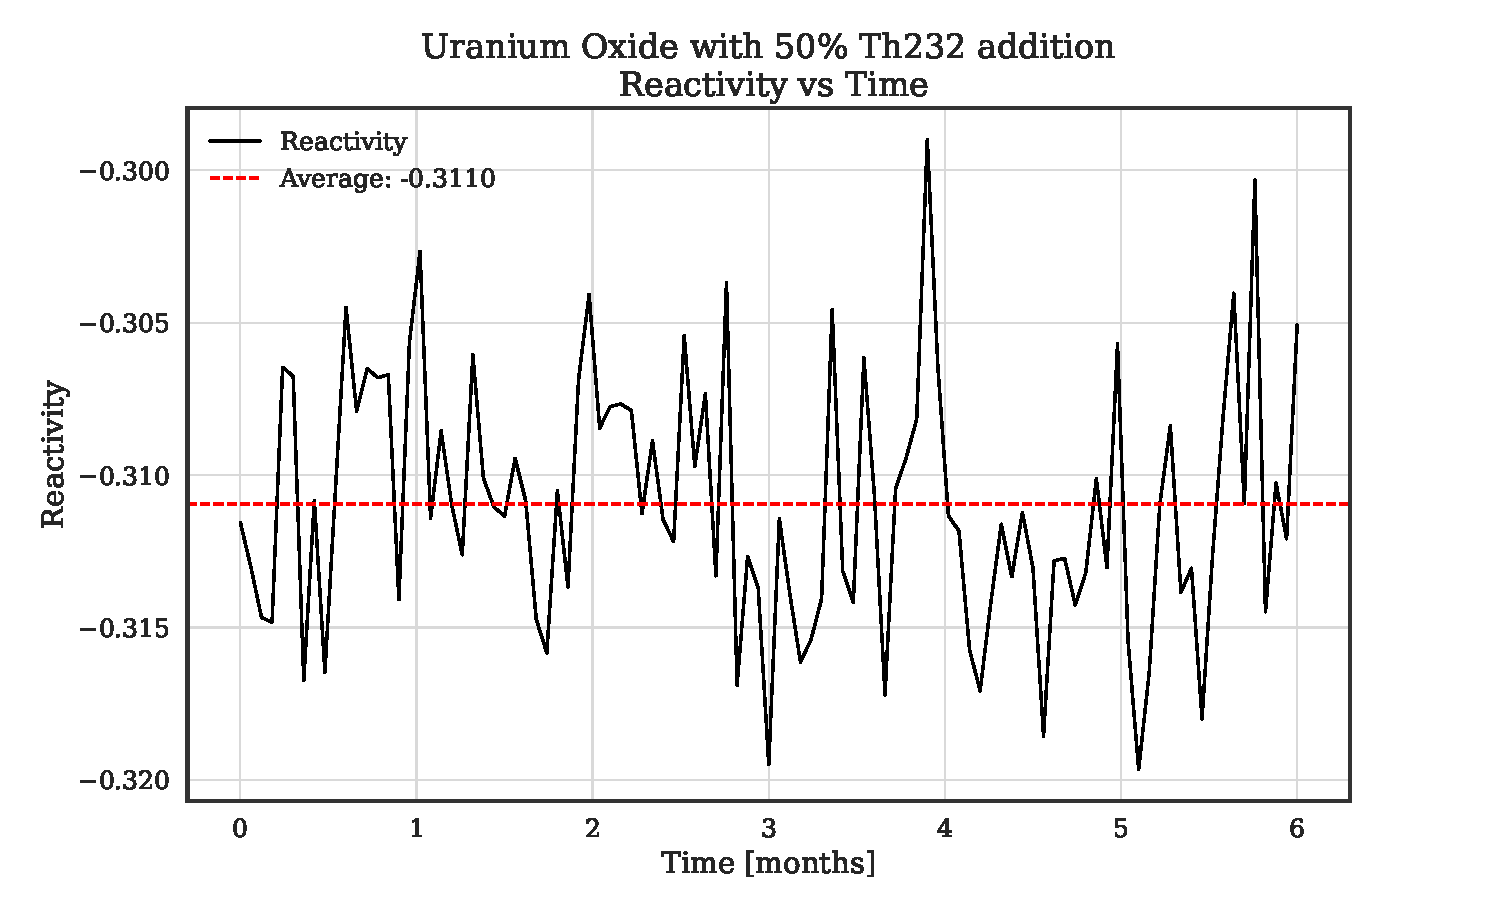
\includegraphics[width=0.75\textwidth, scale = 0.5]{Kap7/Figures_Kap7/Reactivity_vs_Time_UOX_50.pdf}
    \caption{Reactivity over time of the simulation of a PWR fuel assembly using UOX at \(50 \, \%\) thorium concentration.}
    \label{fig:p_10}
\end{figure}

Additional simulations were done to evaluate the behavior of thorium based fuel using thorium oxide and plutonium as seed isotope. The concentration of plutonium was set to \(10 \, \%\). The simulation shows that the fuel assembly reaches a critical state as well as it achieves a breeding ratio of \(\prescript{233}{}{U}\). However, the reactivity of the fuel assembly is higher than \(0\), this implies a more dangerous reactor behavior and additional technical issues to run it safetly. The results are shown in figures \textbf{Fig.}\ref{fig:th_pu}. The behavior of reactivity is show in figure \textbf{Fig.}\ref{fig:p_th_pu}.   

\begin{figure}[h]
    \centering
    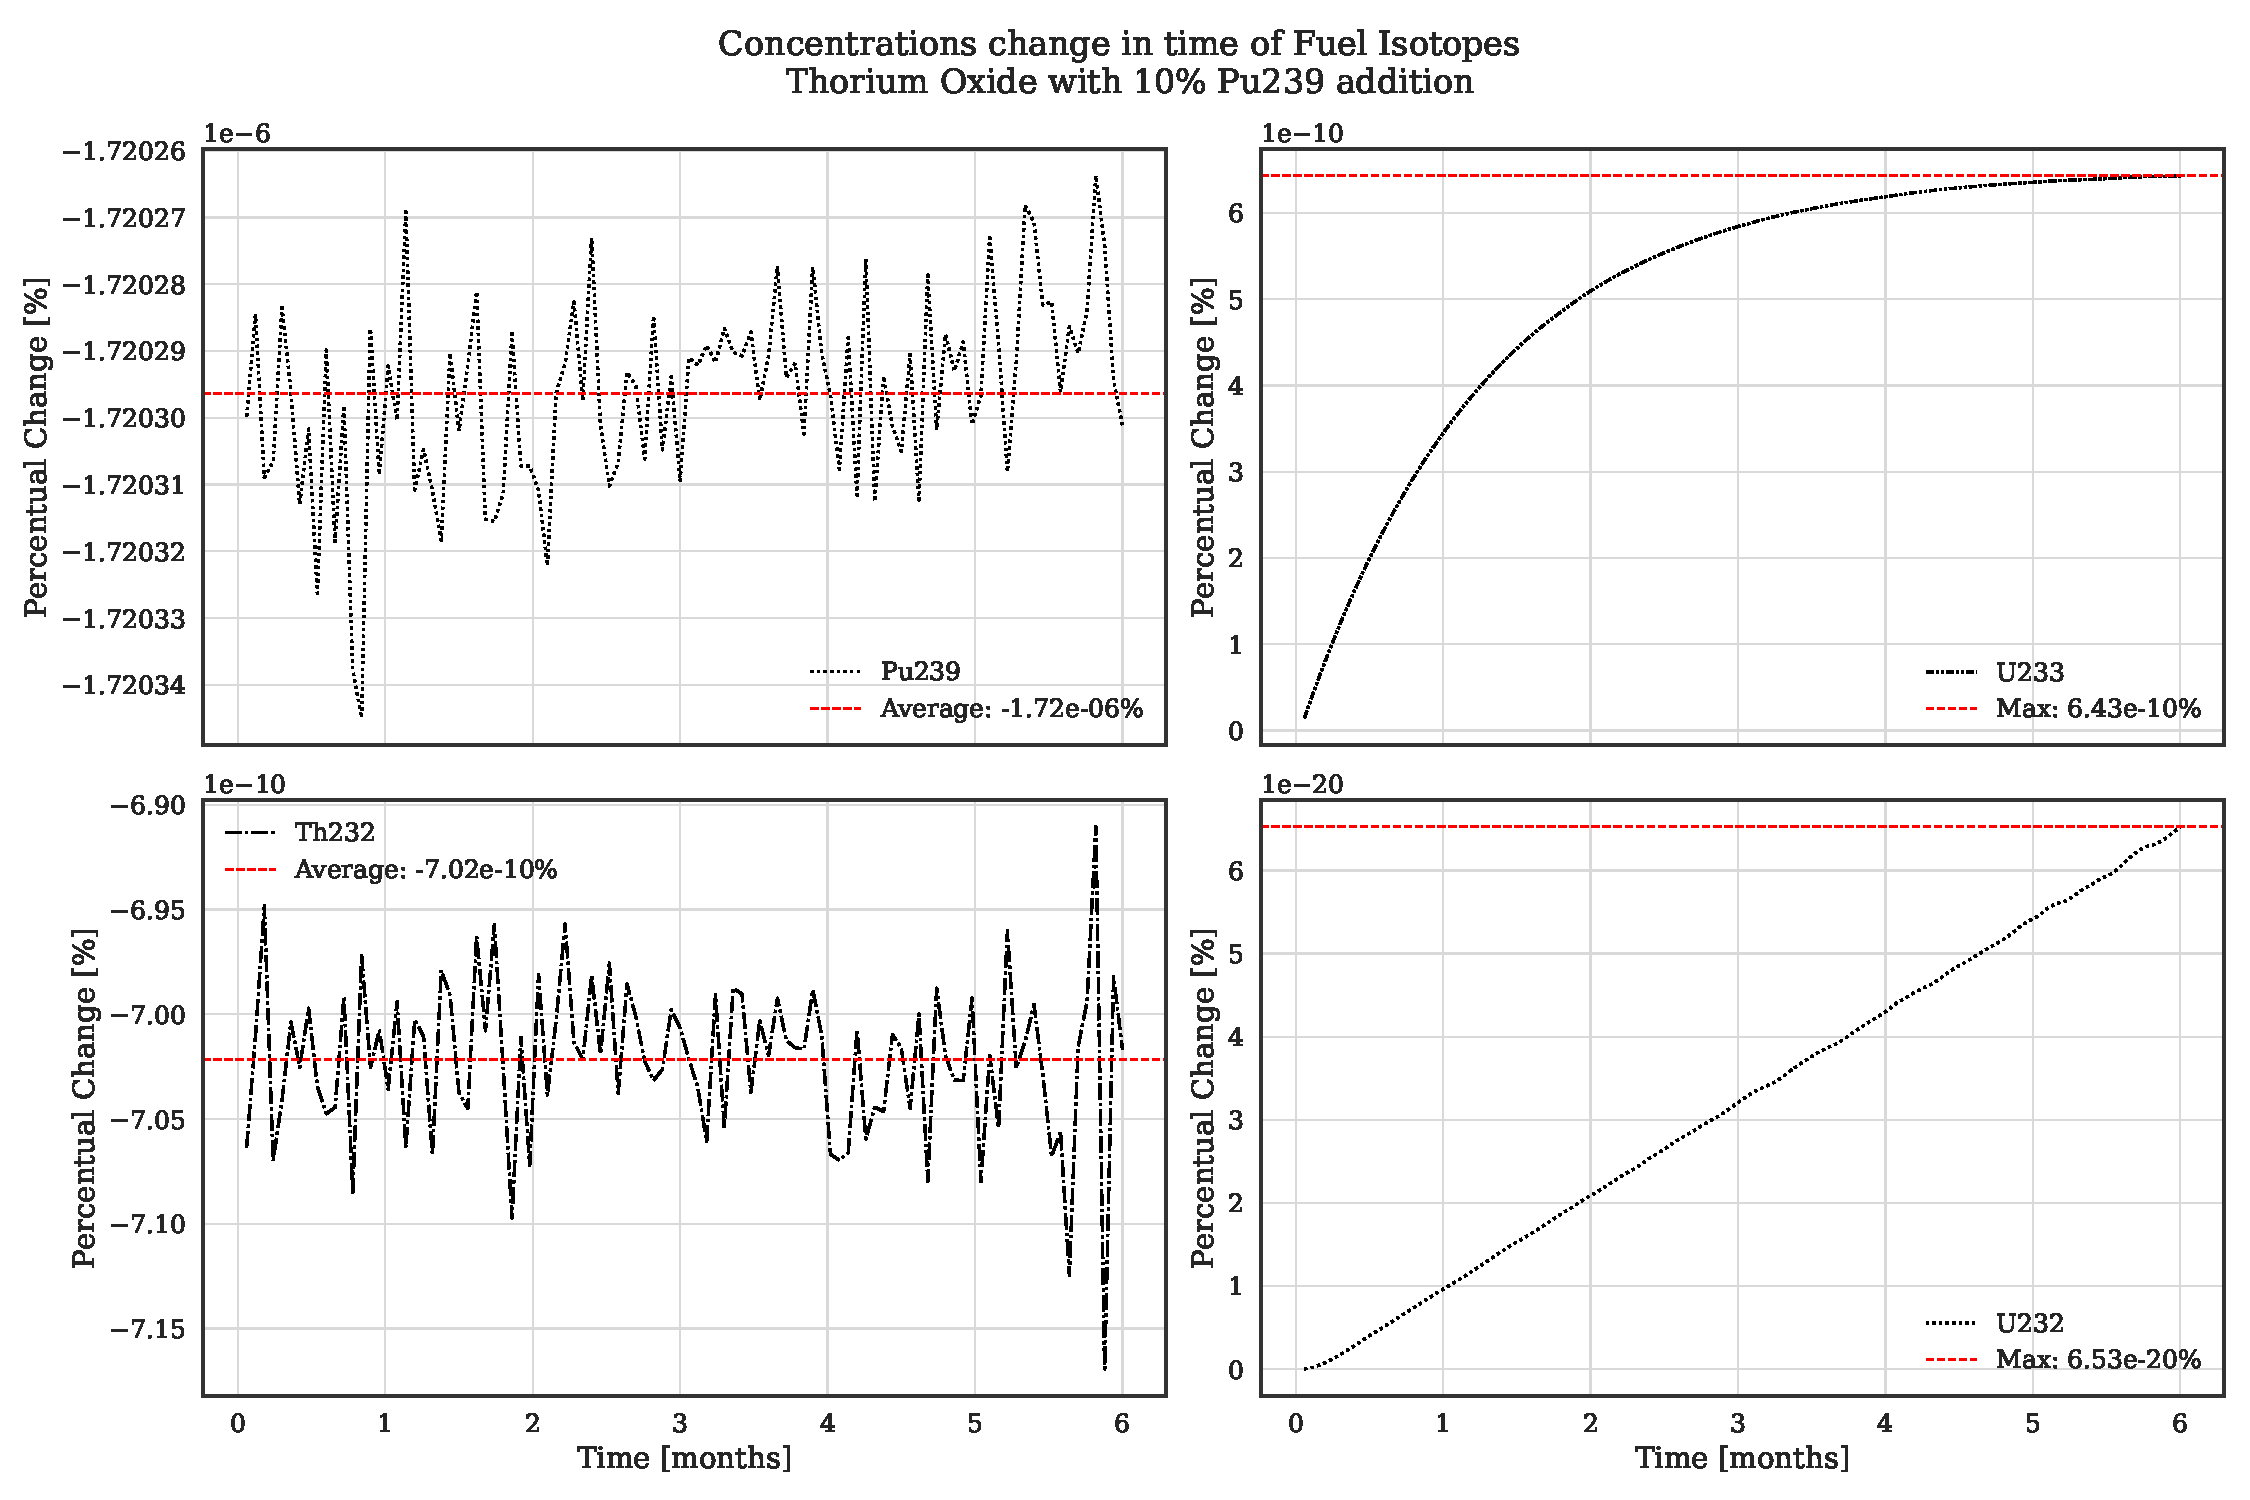
\includegraphics[width=1\textwidth]{Kap7/Figures_Kap7/percentual_change_th232_Pu239.pdf}
    \caption{Percentage change of isotopes in the simulation of a PWR fuel assembly using ThOX and \(10 \, \%\) plutonium concentration.}
    \label{fig:th_pu}
\end{figure}  


\begin{figure}[h]
    \centering
    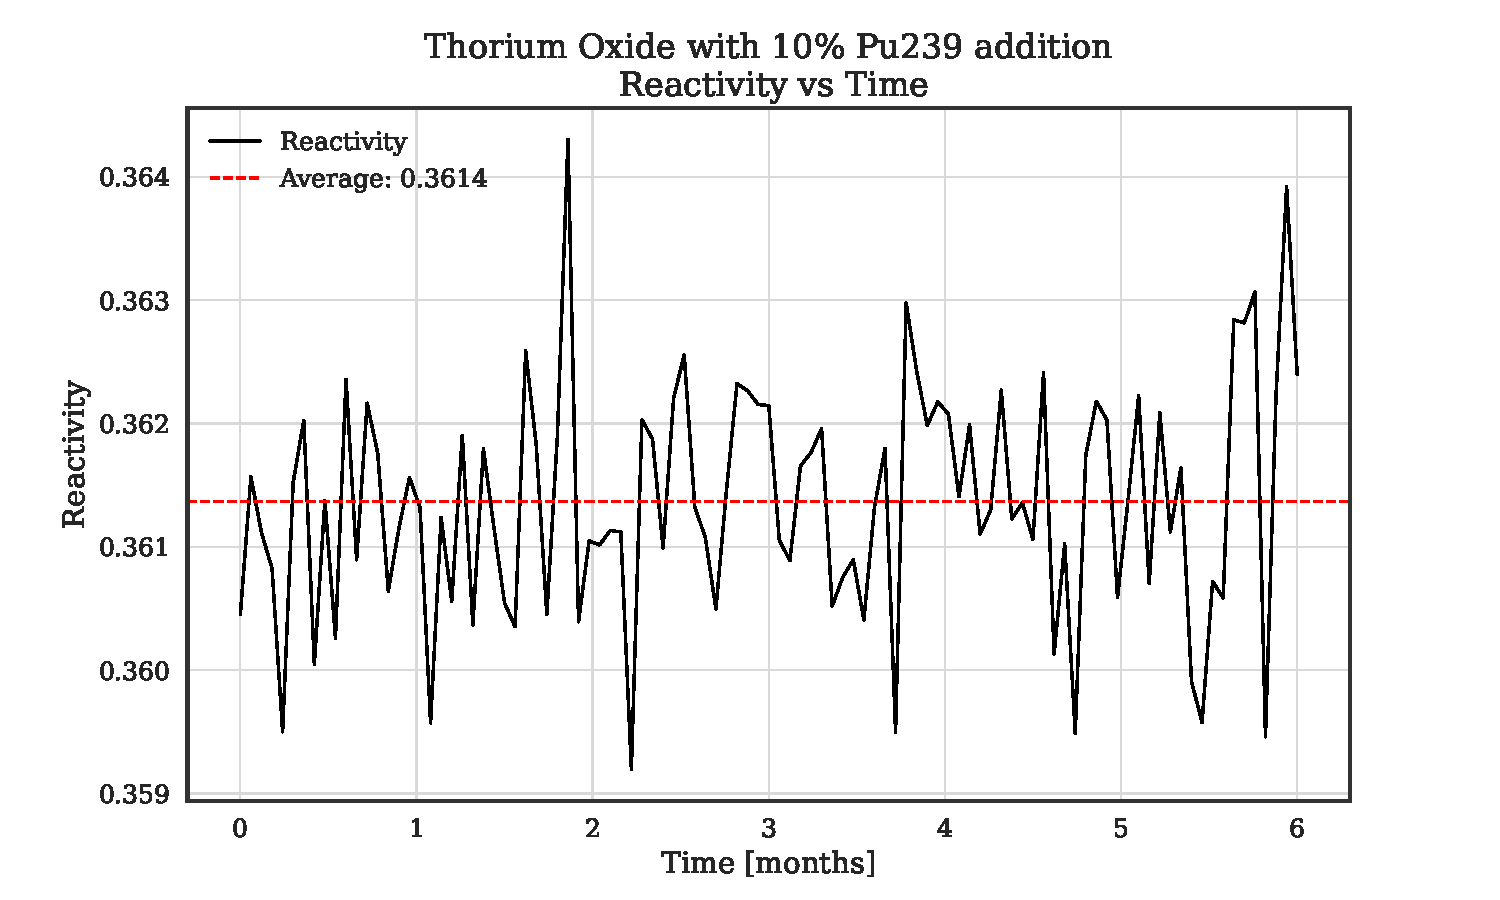
\includegraphics[width=0.75\textwidth, scale = 0.5]{Kap7/Figures_Kap7/Reactivity_vs_Time_ThOX_Pu10.pdf}
    \caption{Reactivity over time of the simulation of a PWR fuel assembly using ThOX and \(10 \, \%\) plutonium concentration.}
    \label{fig:p_th_pu}
\end{figure}

\section{Conclusion}
The simulations conducted in this project provide valuable insights into the behavior of thorium-based nuclear fuels in a Pressurized Water Reactor (PWR). The results demonstrate that thorium oxide (ThOX) with uranium-233 (\(\prescript{233}{}{U}\)) at concentrations of \(5 \, \%\) and \(10 \, \%\) can achieve breeding. However, the stability of breeding is achieved much later compared to plutonium-239 (\(\prescript{239}{}{Pu}\)). This delay is due to the slower breeding process of \(\prescript{233}{}{U}\) from \(\prescript{232}{}{Th}\) compared to the breeding of \(\prescript{239}{}{Pu}\) from \(\prescript{238}{}{U}\).

Additionally, the simulations show an improvement in neutronic economy with thorium-based fuels. This improvement is characterized by a reduction in excess reactivity at the beginning of the fuel cycle, which helps to minimize the initial reactivity spike and associated control challenges. Furthermore, the simulations indicate that thorium-based fuels can maintain criticality towards the end of the fuel cycle, ensuring a more stable and efficient reactor operation over time.Overall, the use of ThOX with \(\prescript{233}{}{U}\) not only supports breeding but also enhances the neutronic performance of the reactor by providing a more balanced reactivity profile throughout the fuel cycle.

The simulation results for ThOX with \(10 \, \%\) thorium concentration (\textbf{Fig.}\ref{fig:th10}) show a good neutronic economy, aligning with previously reported results. However, increasing the thorium concentration to \(50 \, \%\) leads to subcritical reactor behavior (\textbf{Fig.}\ref{fig:th50}). This indicates that while thorium can be beneficial in certain concentrations, higher concentrations may pose challenges for maintaining criticality.

Additionally, the simulation of ThOX with \(10 \, \%\) plutonium concentration (\textbf{Fig.}\ref{fig:th_pu}) shows that the fuel assembly reaches a critical state and achieves a breeding ratio of \(\prescript{233}{}{U}\). However, the higher reactivity of the fuel assembly implies a more dangerous reactor behavior and additional technical issues to ensure safe operation (\textbf{Fig.}\ref{fig:p_th_pu}).

For comparison, the simulation using uranium oxide (UOX) as a reference (\textbf{Fig.}\ref{fig:uo2}) highlights the differences in behavior between traditional uranium-based fuels and thorium-based fuels. The results indicate that while UOX can maintain criticality, the breeding capabilities of thorium-based fuels offer potential advantages for long-term sustainability and fuel utilization.

In conclusion, thorium-based fuels, particularly ThOX with \(\prescript{233}{}{U}\), show promise for use in PWRs. However, while the chain reaction can be sustained with these fuels, the simulations indicate that achieving criticality is challenging, since the reactivity was about \(0\)(), and it was not possible to achieve a stable breeding of \(\prescript{233}{}{U}\). Careful consideration of fuel composition and concentration is necessary to balance breeding capabilities and reactor safety. Further research and optimization are required to fully realize the potential of thorium as a sustainable nuclear fuel.

